\documentclass[12pt,fleqn]{article}

\usepackage[utf8]{inputenc}
\usepackage[T2A]{fontenc}
\usepackage{amssymb,amsmath,mathrsfs,amsthm}
\usepackage[russian]{babel}
\usepackage{graphicx}
\usepackage[footnotesize]{caption2}
\usepackage{indentfirst}
\usepackage{epstopdf}
%\usepackage[ruled,section]{algorithm}
%\usepackage[noend]{algorithmic}
%\usepackage[all]{xy}

\usepackage[ruled,vlined,linesnumbered,algosection,algo2e]{algorithm2e}
% Перевод плагина algorithm2e
\SetKwInput{KwData}{Исходные параметры}
\SetKwInput{KwResult}{Результат}
\SetKwInput{KwIn}{Входные данные}
\SetKwInput{KwOut}{Выходные данные}
\SetKwIF{If}{ElseIf}{Else}{если}{тогда}{иначе\ если}{иначе}{конец\ условия}
\SetKwFor{While}{до\ тех\ пор,\ пока}{выполнять}{конец\ цикла}
\SetKw{KwTo}{от}
\SetKw{KwRet}{возвратить}
\SetKw{Return}{возвратить}
\SetKwBlock{Begin}{начало\ блока}{конец\ блока}
\SetKwSwitch{Switch}{Case}{Other}{Проверить\ значение}{и\ выполнить}{вариант}{в\ противном\ случае}{конец\ варианта}{конец\ проверки\ значений}
\SetKwFor{For}{цикл}{выполнять}{конец\ цикла}
\SetKwFor{ForEach}{для\ каждого}{выполнять}{конец\ цикла}
\SetKwRepeat{Repeat}{повторять}{до\ тех\ пор,\ пока}
\SetAlgorithmName{Алгоритм}{алгоритм}{Список алгоритмов}

% Параметры страницы
\textheight=24cm
\textwidth=16cm
\oddsidemargin=5mm
\evensidemargin=-5mm
\marginparwidth=36pt
\topmargin=-1cm
\footnotesep=3ex
%\flushbottom
\raggedbottom
\tolerance 3000
% подавить эффект "висячих стpок"
\clubpenalty=10000
\widowpenalty=10000
\renewcommand{\baselinestretch}{1.1}
\renewcommand{\baselinestretch}{1.5} %для печати с большим интервалом

\begin{document}

\begin{titlepage}
\begin{center}
    Московский государственный университет имени М. В. Ломоносова

    \bigskip
    
\includegraphics[width=50mm]{msu.eps}

    \bigskip
    Факультет Вычислительной Математики и Кибернетики\\
    Кафедра Математических Методов Прогнозирования\\[10mm]

    \textsf{\large\bfseries
        ДИПЛОМНАЯ РАБОТА СТУДЕНТА 517 ГРУППЫ\\[10mm]
        <<Управление динамическим объектом с использованием нейрокомпьютерного интерфейса>>
    }\\[10mm]

    \begin{flushright}
        \parbox{0.5\textwidth}{
            Выполнил:\\
            студент 5 курса 517 группы\\
            \emph{Зиннурова Эльвира Альбертовна}\\[5mm]
            Научный руководитель:\\
            к.ф-м.н., доцент\\
            \emph{Гуров Сергей Исаевич}
        }
    \end{flushright}

    \begin{tabular}{p{0.45\textwidth}p{0.45\textwidth}}
        Заведующий кафедрой\newline
        Математических Методов\newline
        Прогнозирования, академик РАН
        &
        ~\newline~\newline
        \hfill\hbox to 0.45\textwidth{\hrulefill~Ю. И. Журавлёв}
    \\[20mm]
        К защите допускаю\newline
        \hbox to 0.4\textwidth{<<\hbox to 12mm{\hrulefill}>> \hrulefill~2015 г.}
        &
        К защите рекомендую\newline
        \hbox to 0.45\textwidth{<<\hbox to 12mm{\hrulefill}>> \hrulefill~2015 г.}
    \end{tabular}

    \vspace{\fill}
    Москва, 2015
\end{center}
\end{titlepage}

\newpage
\renewcommand{\contentsname}{Содержание}
\tableofcontents

\newpage
\begin{abstract}
    Данный документ является образцом оформления дипломной работы для студентов кафедры 
    Математических методов прогнозирования ВМК~МГУ. 
    Приведённые ниже рекомендации взяты из~статьи
    <<Написание отчётов и статей (рекомендации)>>
    на~вики"~ресурсе \texttt{www.MachineLearning.ru}.
    Студенты, готовящие дипломную работу к~защите, 
    могут найти много полезной информации также в~статьях 
    <<Научно-исследовательская работа (рекомендации)>>,
    <<Подготовка презентаций (рекомендации)>>,
    <<Защита выпускной квалификационной работы (рекомендации)>>
    на~том~же ресурсе. 

    Аннотация обычно содержит 
    краткое описание постановки задачи и~полученных результатов,
    одним абзацем на 10--15 строк.
    Цель аннотации "--- обозначить в~общих чертах, о~чём работа,
    чтобы человек, совершенно не~знакомый с~данной работой,
    понял, интересна~ли ему эта тема, и~стоит~ли читать дальше.
    Аннотация собирается в~последнюю очередь
    путем легкой модификации наиболее важных и~удачных фраз из введения и~заключения.
\end{abstract}

\newpage
\section{Введение}
	\quad\,\,\,Нейрокомпьютерный интерфейс (англ. {\it brain-computer interface, mind-machine interface, brain–machine interface}, интерфейс «мозг-компьютер», зачастую используется сокращение {\it BCI}) ~--- специальный вид интерфейса, созданный для обмена информацией между мозгом и средствами вычислительной техники. Одной из задач, стоящих перед исследователями, работающими в данной области, является создание устройств, которые позволят людям с утраченными способностями организма полноценно взаимодействовать с окружающим миром. Управление объектами реального мира при помощи ментальных команд может открыть новые возможности для парализованных людей. 
	\par В последние годы ведётся активная разработка различных практических приложений с использованием интерфейса «мозг-компьютер». Многие исследовательские группы по всему миру занимаются тематикой BCI, и в разработке многих направлений тематики имеются заметные успехи, однако до сих пор существует масса сложностей в практическом применении нейрокомпьютерного интерфейса.
	\par TODO: В данной работе рассматриваются методы того-то и того, приведено то-то и то-то, расписать по главам... (в последнюю очередь)

\clearpage 

\section{Постановка задачи}
	\quad\,\,\,Целью данной работы является построение модели нейрокомпьютерного интерфейса для управления движением динамического объекта в некотором направлении с использованием доступного устройства {\it Emotiv EPOC}. Каждому из рассматриваемых направлений соответствует некоторая метка класса.
 	\par Пусть имеется $M$ сенсоров, в моменты времени $1, 2, \dots, t, \dots$ $i$-ый сенсор фиксирует значения $x^i(t)$, $i = \overline{1,M}.$ Требуется определить класс регистрируемого в произвольный момент времени $t$ сигнала. Зачастую полагают, что многомерный сигнал разбит на отрезки известной длины $T$, на протяжении каждого из которых класс сигнала остаётся неизменным. Везде далее будем придерживаться данного предположения.
	\par Дадим формальную математическую постановку задачи.
	\par Имеется пространство объектов $\mathcal{X} \subset \mathbb{R}^{M \times T}$, каждый из которых представляет собой сигнал, зафиксированный при помощи $M$ сенсоров в течение периода времени длины $T$, и конечное множество имён классов $\mathcal{Y}, \, |\mathcal{Y}| = N$. Существует целевая зависимость $y^*: \mathcal{X} \to \mathcal{Y},$ значения которой известны только на объектах обучающей выборки $X^L = \{ (x^i, y^i)\}_{i=1}^L, \, x^i \in \mathcal{X} \subset \mathbb{R}^{M \times T}, \, y^i = y^*(x^i) \in \mathcal{Y}, \, L$ -- количество объектов обучающей выборки. Требуется построить алгоритм классификации $a: \mathcal{X} \to \mathcal{Y},$ аппроксимирующий целевую зависимость $y^*(x)$ на всем множестве $\mathcal{X}$ в соответствии с некоторым введённым функционалом качества.

\clearpage 

\section{Введение в нейрокомпьютерные интерфейсы}
	\subsection{Используемое оборудование}
	\par Главная цель исследований в области нейрокомпьютерных интерфейсов -- разработка систем, позволяющих обездвиженным пользователям обмениваться информацией и взаимодействовать с другими людьми, а также контролировать различные элементы их окружения. Кроме того, подобные системы могут быть использованы для улучшения контроля над сложными многозадачными операциями.
	\par Нейрокомпьютерный интерфейс -- средство коммуникации, транслирующее активность головного мозга в действия либо команды для электронных устройств. Фиксация подобного рода активности становится возможной вследствие физико-химических процессов, лежащих в основе обмена веществ в нервной ткани, порождающих колебания потенциалов головного мозга. Несмотря на то что существует множество различных методов фиксации активности головного мозга (электрокортикограмма, электроокулограмма и др.), в настоящее время основным способом получения сигнала головного мозга является электроэнцефалограмма. 
	\par {\it Электроэнцефалография (ЭЭГ)} — раздел электрофизиологии, изучающий закономерности суммарной электрической активности мозга, отводимой с поверхности кожи головы или мозга, а также метод записи таких потенциалов. Получение электроэнцефалограммы осуществляется с помощью электроэнцефалографа. Существуют различные устройства для записи ЭЭГ, отличающиеся следующими характеристиками: 
	\begin{itemize}\itemsep0pt
	\item
	характеристики принимающего сигнала (частота, количество шума в сигнале);
	\item
	инвазивность (степень имплантирования электродов в кору головного мозга);
	\item
	количество электродов;
	\item
	покрываемая площадь (среднее количество влияющих на сигнал нейронов, снимаемых одним электродом).
	\end{itemize}
	\par По инвазивности устройства делятся на {\it погружные}, {\it частично-погружные} и {\it непогружные} в зависимости от расположения электродов (электроды вживлены в мозг/сращены с нервами, находятся на поверхности мозга/рядом с нервами или находятся на поверхности кожи головы соответственно).

	\par Устройства с непогружным интерфейсом делятся на {\it мокрые} и {\it сухие} в зависимости от того, необходимо ли смачивание электродов проводящей жидкостью для осуществления контакта.
	\par По типу электродов устройства делятся на {\it пассивные} и {\it активные} в зависимости от того, проивзодится ли после снятия электродом сигнала его первичная обработка.

	
	\par В настоящей работе для записи электроэнцефалограммы использовалось устройство {\it Emotiv EPOC}. Это устройство было разработано австралийской компанией {\it Emotiv Systems}, основанной в 2003 году. Данная компания входит в число трёх основных участников рынка потребительских устройств BCI наряду с компаниями {\it NeuroSky} и {\it OCZ}, однако {\it Emotiv EPOC} имеет значительно большее число электродов, чем устройства компаний-конкурентов, и незначительно более высокую стоимость. 
\begin{figure}[h!]
\center{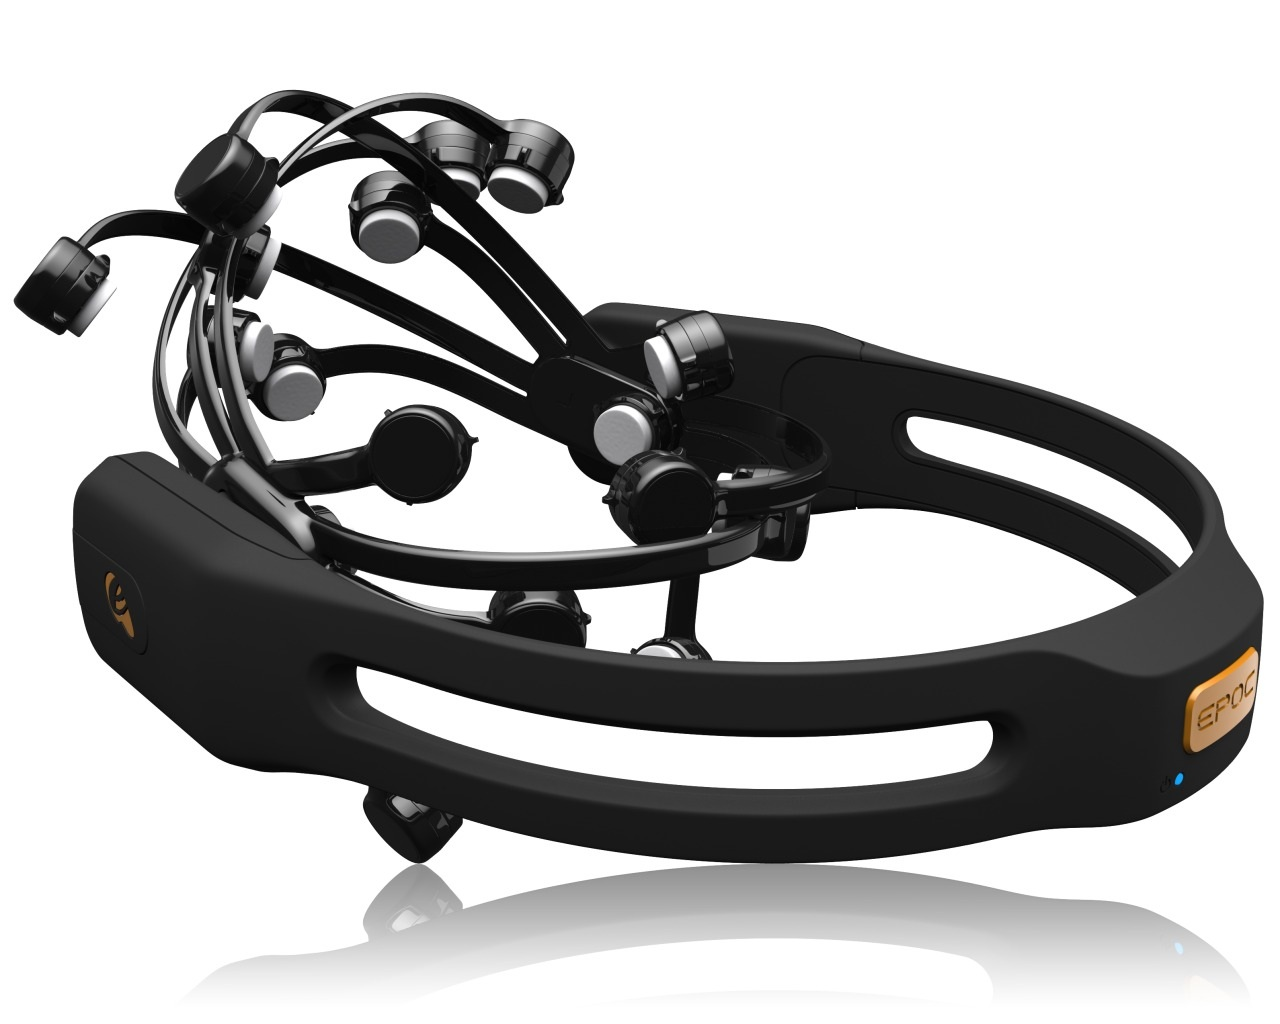
\includegraphics[width=1\linewidth]{Emotiv.jpg}}
\caption{{\it Emotiv EPOC} ~--- устройство, используемое для записи данных.}
\label{Emotiv}
\end{figure}

	\par Общий вид устройства изображён на рис.~\ref{Emotiv}, устройство обладает следующими характеристиками:
	\begin{itemize}\itemsep0pt
	\item
	число датчиков — 14;
	\item
	тип датчиков — пассивные, мокрые;
	\item
	частота дискретизации — 128 Гц;
	\item
	способ связи — беспроводная радиосвязь;
	\item
	гироскопы — 2 шт.;
	\item
	инвазивность — непогружной.
	\end{itemize}

	\par Расположение электродов согласно международной системе размещения электродов <<10 -- 20>> изображено на рис.~\ref{electrode_map}.
	\par Устройство {\it Emotiv EPOC} было использовано в силу своей доступности. Также достоинствами данного устройства являются портативность, простота использования и небольшие размеры. В то же время оно обладает и рядом недостатков: низкая точность снимаемого сигнала и ненадёжная фиксация устройства на голове человека. В рамках настоящей работы будет предпринята попытка купировать недостатки устройства применяемыми методами обработки и классификации сигнала.

	\begin{figure}[h!]
	\center{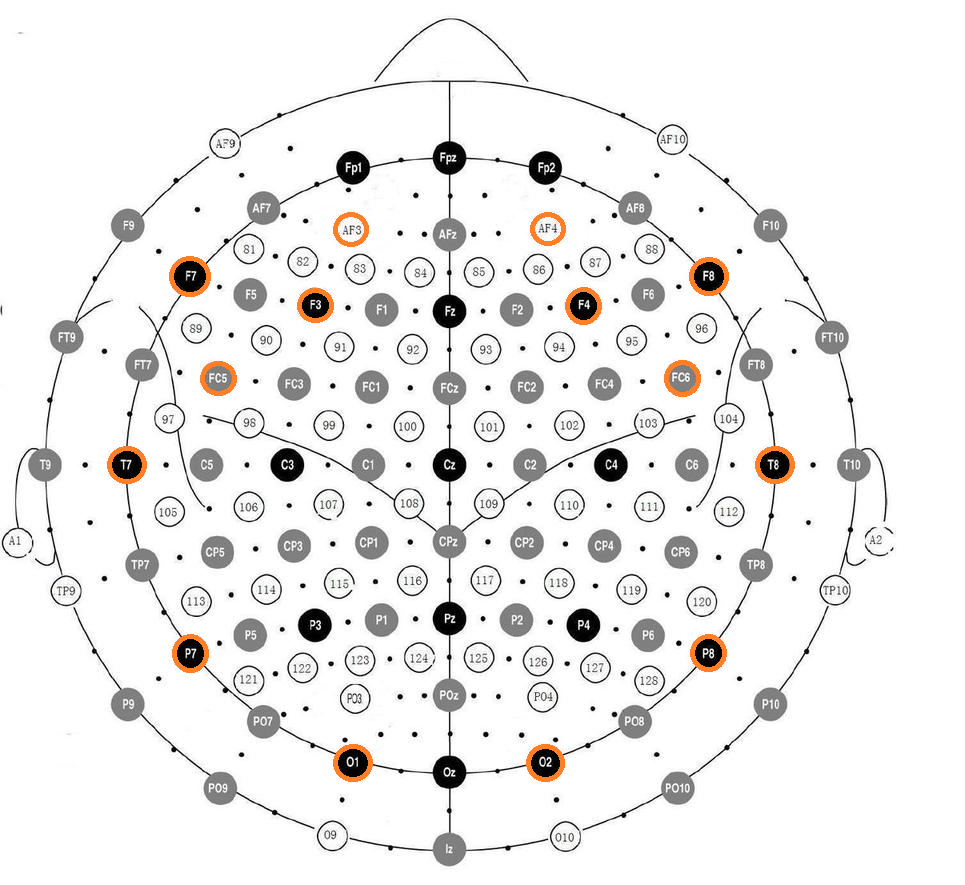
\includegraphics[width=0.9\textwidth]{electrode_map_1020.png}}
		\caption{Расположение электродов на голове человека согласно международной системе размещения электродов <<10--20>>. Электроды устройства {\it Emotiv EPOC} выделены оранжевым цветом.}
	\label{electrode_map}
	\end{figure}

	\subsection{Типы нейрофизиологических сигналов}
	\par Предполагается, что идеальный нейрокомпьютерный интерфейс будет напрямую транслировать каждое намерение пользователя и выполнять соответствующее действие. Однако чётко определение того, как соотносятся друг с другом намерения пользователя и нейрофизиологические сигналы, является нетривиальной задачей. На сегодняшний день это является одной из основных причин ограниченности свободы действий в существующих системах BCI.
	\par TODO: Про частоты?
	\par Для возможности распознавания различных нейрофизиологических сигналов и возможности сопоставления подобного рода сигналов и подразумеваемых действий необходимо осознанное управление активностью головного мозга. В основном, для достижения этой цели используются два подхода. При использовании первого подхода испутыемые должны наблюдать набор стимулов нейрокомпьютерного интерфейса, и контроль мозговой активности осуществляется путём концентрации на одном конкретном стимуле. Изменения в нейрофизиологических сигналах в результате различий между стимулами называются {\it вызванными потенциалами} (англ. event-related potentials, ERPs). При использовании второго подхода пользователи управляют мозговой активностью путём концентрации на определённом ментальном задании, например, представление определённого движения руки может быть использовано для изменения активности в соответствующей части скальпа.
		\subsubsection{Вызванные потенциалы}
	\par Вызванный потенциал — электрическая реакция мозга на внешний раздражитель или на выполнение умственной (когнитивной) задачи. Потенциалы данного вида имеют место в течение определённого промежутка времени после наблюдения стимула.
	\begin{itemize}
	\item
	{\bf Волны P300}
	\par Волна P300 -- положительное отклонение сигнала ЭЭГ, имеющее место ориентировочно через 300 мс после демонстрации редко появляющегося стимула, связанного с некоторым заданием. Для порождения подобного рода волн испытуемый должен пронаблюдать последовательность двух видом стимулов. Первый тип стимулов (т.н. {\it целевые} стимулы) являются редкими в последовательности стимулов, в то время как стимулы другого типа (т.н. {\it отвлекающие} стимулы) являются более частыми. Таким образом, во время появления целевого стимула может быть зафиксирована мозговая активность, содержащая волны P300. Данный принцип был использован (фарвелл и дончин) в разработанной ими системе BCI. В их исследовании было описано устройство для набора текста. На экране изображалась таблица доступных для набора символов, строки и столбцы которой выделялись в случайном порядке, в качестве целевого стимула выступало выделение столбца/строки с желаемым на данный момент символом, отвлекающих стимулов - выделение остальных столбцов/строк.
	\item
	{\bf Steady-State Visual Evoked Potentials (SSVEPs)}
	\par SSVEPs -- осцилляции, имеющие место в данных, полученных при помощи затылочных сенсоров, могут быть индуцированы путём наблюдения часто повторяющейся анимации. Подобного рода стимуляция порождает колебания той же частоты в регистрируемых сигналах головного мозга. В исследованиях по тематике нейрокомпьютерных интерфейсов потенциалы этого типа используются при одновременной демонстрации стимулов с разной частотой. Таким образом, пользователь путём концентрации на конкретном стимуле имеет возможность управлять мозговой активностью.
	\item
	{\bf Motor-Related Potentials (MRPs)}
	\par MRPs -- продолжительные отрицательные потенциалы, связанные с ожиданием или ментальным представлением выполняемого движения или действия, имеют место в сенсомоторной части скальпа в начале выполнения движения или в процессе ментального представления движения.
	\end{itemize}
		\subsubsection{Частотная мозговая активность}
	\par В электроэнцефалограмме здорового человека выделяют несколько характерных составляющих электрических колебаний, называемых ритмами, различающихся частотным диапазоном, а также амплитудой, формой волны и другими характеристиками. Считается, что каждый ритм соответствует некоторому определённому состоянию мозга и связан с определёнными церебральными механизмами.
	\par TODO: таблица частот для ритмов
	\begin{itemize}
	\item
	{\bf Сенсомоторные ритмы}
	\par Колебания $\mu$-ритма могут быть обнаружены в сенсомоторной части сальпа, когда пользователь не выполняет никаких действий. Если же движение некоторой части тела выполняется или выполняется ментальное задание по представлению данного движения, амплитуда колебаний уменьшается. Кроме того, представляемые или выполняемые движения порождают изменения в амплитуде $\beta$-ритма. Изменения данных ритмов отражаются на части скальпа, отвечающей перемещаемой части тела, в связи с этим представляемые и выполняемые движения различных частей тела могут быть отличимы друг от друга. Происходящие изменения для пользователей с небольшим опытом использования нейрокомпьютерных интерфейсов обычно оказываются недостаточно весомыми для адекватного функционирования распознающих алгоритмов.
	\item
	{\bf Другая активность}
	\par В качестве триггеров возникновения колебаний потенциалов могут быть использованы когнитивные задания, отличные от представления движений, например, вычисления, слуховые представления, представление движения трёхмерного объекта в пространстве и др.
	\end{itemize}
	\subsection{Нейрокомпьютерные интерфейсы на основе волн P300}
	\subsubsection{Вызванные потенциалы и волны P300}
	\par Волны P300 были открыты в исследовании .... С тех пор имело место множество исследований по изучению природы этих колебаний путём изменения различных характеристик проводимых экспериментов, таких как способ демонстрации стимула, пол, возраст испытуемых, наличие заболеваний  и пр.
	\par Различные парадигмы могут быть использованы для выявления волн P300. В качестве стимулов могут быть использованы слуховые, визуальные, тактильные, обонятельные, вкусовые стимулы. Тем не менее, в силу практичности чаще всего используются визуальные и слуховые стимулы, а также сочетание обоих. В основном в большинстве исследований применяются две парадигмы: оригинальная (oddball paradigm) и трёхстимульная (three-stimulus).
	\par Оригинальная парадигма подразумевает использование двух стимулов (целевого и отвлекающего), демонстрируемых в произвольном порядке, причём демонстрация целевого стимула является гораздо более редким событием по сравнению с демонстрацией отвлекающего стимула. Испытуемымому же необходимо концентрироваться исключительно на целевом стимуле и игнорировать появление отвлекающего стимула.
	\par Трёхстимульная парадигма является модификацией оригинальной парадигмы. В данном случае также присутствиет так называемый Оотвлекающий стимул, редко появляющийся в последовательности целевых и нецелевых стимулов. Испытуемые не информируются о наличии подобного рода стимула в процессе инструктажа.
	\par При использовании описанных парадигм наблюдаются различные типы волн P300. Применение оригнальной парадигмы позволяет обнаружить т.н. волны P3b, имеющие место в течение 300-500 мс, только если пользователь концентрируется на стимуле. Если же пользователь не уделяет внимание стимулу, целевой стимул при ипользовании оригинальной парадигмы порождает другой тип волны P300, называемый P3a, имеющие место в течение 200-400 мс. При применении трёхстимульной парадигмы целевой стимул также порождает волны P3b, Отвлекающий же стимул порождает волны P3a. Отношение между каждой из парадигм и описанными типами волн P300 изображены на на рис.~\ref{paradigms}.

\begin{figure}[h!]
\begin{minipage}[h!]{0.47\linewidth}
\center{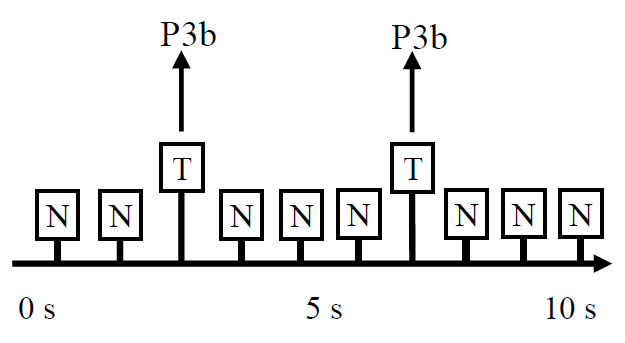
\includegraphics[width=1\linewidth]{oddball.png} \\ а)}
\end{minipage}
\hfill
\begin{minipage}[h!]{0.52\linewidth}
\center{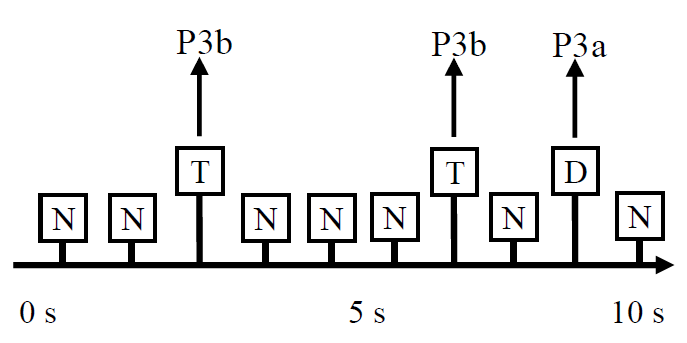
\includegraphics[width=1\linewidth]{3stim.png} \\ б)}
\end{minipage}
\caption{Оригинальная (а) и трёхстимульная (б) парадигмы проведения экспериментов с порождением волн P300.}
\label{paradigms}
\end{figure}

	\subsubsection{Факторы, влияющие на ...}
	\par Кроме влияния различных экспериментальных парадигм, упомянутых выше, волны P300 также подвергаются влиянию многих других факторов? пtречисленных ниже:
	\begin{itemize}
	\item
	{\bf Веростность появления целевого стимула}
	\par Амплитуда волны P3b обратно пропорциональна вероятности появления целевого стимула: редкое появление целевого стимула порождает высокий пик волны, в то время как высокая вероятность появления стимула слабо отражается на сигнале. В основном при проведении экспериментов используется вероятность, примерно равная 10\% для более надёжного выявления волн P300.  Кроме того, на амплитуду волны P3b также влияет локальная вероятность появления целевого стимула.
	\item
	{\bf Межстимульный интервал}
	\par Амплитуда волны P3b прямо пропорциональна продолжительности межстимульного интервала (период времени между двумя последовательными стимулами).
	\item
	{\bf Привыкание}
	\par Амплитуда волны P3a снижается с течением времени, поскольку из-за демонстрации большого количества Отвлекающих стимулов данное событие становится ожидаемым для испытуемого. В то же время амплитуда волны P3b практически не подвержена влиянию этого фактора.
	\item
	{\bf Внимание}
	\par Амплитуда волны P3b в большой мере зависит от степени концентрации пользователя. Более детально, волны P3b полностью исчезают, если пользователь не вовлечен в активное выполнение заданий. В то же время волны P3a не подвергнуты влиянию данного фактора.
	\item
	{\bf Сложность заданий}
	\par Латентность волны P3b прямо пропорциональна сложности выполняемного  задания, в то время как амплитуда обратно пропорционально этой величине. К примеру, целевые стимулы, сильно отличающиеся от нецелевых, ведут к более высокой амплитуде волны P3b по сравнению со случаем слабых отличий между целевыми и нецелевыми стимулами.  Другой эффект наблюдается для волн P3a. Повышение сложности вычленения целевых и нецелевых стимулов в трёхстимульной парадигме ведёт к повышению амплитуды волн P3a.
	\end{itemize}
	\par TODO: выводы про P3a и P3b?

%	\par TODO: Нужен ли отдельный раздел для Хиперы? Если да, то как назвать этот раздел и раздел про Хиперу?
%	\par В качестве динамического объекта, приводимого в движение при помощи ментальных команд, было использовано устройство {\it Khepera II}. Данное устройство было разработано швейцарской компанией {\it K-team Corporation}.
%	\par Устройство оснащено двумя моторами, приводящими в движение колёса по бокам робота. Устройство управляется путём осуществления команд установки либо изменения скоростей вращения каждого из моторов. (TODO: Нужно ли писать детали о том, как подключается робот к компьютеру, какими командами управляется и т.д.?) Таким образом, имеется возможность осуществления прямолинейного движения либо поворота устройства в плоскости его движения, тем самым команды поворота по и против часовой стрелке на фиксированный угол относительно текущей траектории позволяют управлять движением устройства на плоскости без остановки. Если же, помимо того, использовать команды начала движения и остановки устройства, появится возможность полного управления устройством при движении на плоскости.

\section{Методы распознавания данных ЭЭГ}
	\par TODO: Вставить ссылки на источники
	\par После получения данных при помощи электроэнцефалографа необходимо применение алгоритма, позволяющего определить желаемое для пользователя действие. Входными данными для этого алгоритма являются сигналы ЭЭГ, регистрируемые в процессе демонстрации стимулов.В большинстве существующих на текущий момент исследований по данной тематике задача классификации сигналов разбивается на три большие подзадачи: предобработка сигнала (в целях удаления шумовых компонент), формирование признакового пространства и классификация объектов в построенном признаковом пространстве. Необходимо отметить, что наибольшее влияние на итоговое качество классификации оказывает влияние то, насколько успешно была решена задача формирования признакового пространства. Общая схема работы нейрокомпьютерных интерфейсов представлена на рис.~\ref{bci}.

	\begin{figure}[h!]
	\center{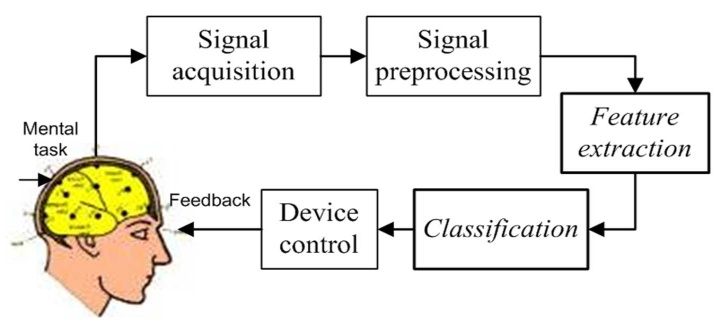
\includegraphics[width=0.9\textwidth]{bci.png}}
	\caption{Общая схема работы нейрокомпьютерных интерфейсов.}
	\label{bci}
	\end{figure}

	\subsection{Предобработка}
	\par Предобработка сигнала проводится с целью удаления артефактов (спонтанные сокращения мышц, моргание и т.п.), а также нейтрализации имеющихся шумовых компонент. Кроме того, зачастую интересующая информация содержится в определённом диапазоне частот, а остальные компоненты являются малоинформативными.
	\begin{itemize}
	\item {\bf Удаление постоянного амплитудного смещения}
	\par {\it Постоянное амплитудное смещение} или {\it DC offset} (англ. {\it direct current offset}, постоянное смещение потока) ~--- отклонение волновой формы относительно оси нулевого уровня сигнала. Амплитудное смещение, наблюдаемое в электроэнцефаллограмме, может быть разложено на две основные составляющие: постоянное смещение, возникающее из-за технических особенностей передачи данных, и  смещение, возникающее из-за взаимодействия электрической цепи с потенциалом тела.
	\item {\bf Полосовая фильтрация}
	\par Как было упомянуто выше, в электроэнцефалограмме здорового человека выделяют несколько характерных составляющих электрических колебаний, называемых ритмами, различающихся частотным диапазоном. С целью выявления компонент, отвечающих соответствующим ритмам, применяются методы фильтрации в заданном диапазоне частот. Диапазон частот выбирается, исходя из априорной информации о ритмах. К примеру, для выделения компоненты, отвечащей за воображаемые движения различных частей тела, используется диапазон $\mu$-ритма (8--13 Гц).
	\par Фильтрами нижних частот называется тип фильтров, эффективно пропускающих частотный спектр сигнала ниже некоторой частоты (т.н. частоты среза) и уменьшающий (подавляющий) частоты сигнала выше этой частоты. Степень подавления каждой частоты зависит от вида фильтра. Фильтр верхних частот, напротив, пропускает частоты выше частоты среза и подавляет низкие частоты.
	\item {\bf Windsorization}
	\par С целью снижения влияния артефактов, имеющих место в данных ЭЭГ, таких как моргание, движения глаз, мышечная активность и др., может применяться ... данных с каждого электрода. Для каждого электрода вычисляются значения перцентилей среза (см. рис. ~\ref{windsorization}), затем значения, лежащие ниже или выше перцентилей среза замещаются соответствующими значениями.

	\begin{figure}[h!]
	\center{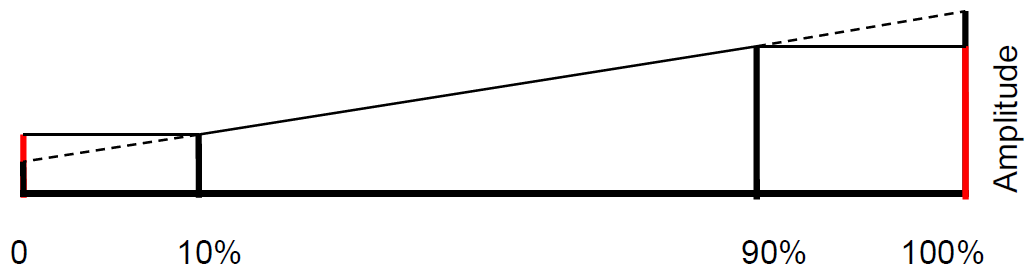
\includegraphics[width=0.9\textwidth]{windsorization.png}}
		\caption{Data windsorization.}
	\label{windsorization}
	\end{figure}

	\item {\bf Отбор электродов}
	\par Современные электроэнцефалографы оснащены десятками электродов, однако информация, получаемая при помощи такого количества сенсоров, является избыточной. Кроме того, увеличение числа электродов ведёт к повышению стоимости устройства и времени на подготовку к использованию, что является недопустимым для электроэнцефалографов, разработанных для коммерческого использования. В связи с этим в современных исследованиях по тематике нейрокомпьютерных интерфейсов наиболее распространены два подхода к решению данной проблемы:
	\begin{enumerate}
	\item выбор электродов с учётом априорных знаний о локализации компонент сигнала на скальпе;
	\item использование методов отбора признаков.
	\end{enumerate}
	\end{itemize}
	\subsection{Построение признакового пространства}
	\par Применение классических методов распознавания в классе задач нейрокомпьютерных интерфейсов не представляется возможным в силу множества причин, среди которых высокая степень зашумлённости данных, высокая размерность пространства, а также многомерность самих сигналов и т.п. В связи с этим этап построения признакового пространства является самым важным в процессе решения задачи. Проблема заключается в том, что не существует единого метода поиска нового признакового пространства. Каждый исследователь сталкивается с необходимостью поиска признакового пространства для эффективного решения конкретной поставленной задачи с использованием конкретного оборудования. 
	\subsubsection{Blind source separation}
	\par Семейство методов BSS основаны на предположении о том, что регистрируемые сигналы для мультиканального устройства являются сместь различных источников сигнала, и являются попыткой выделить исходные источники, преобразуя зарегистрированные сигналы. Классическим примером задачи, иллюстрирующей функциональность данных методов, яволяется "задача коктейльной вечеринки" (cocktail party problem). Предполагается, что снимаемые сигналы $X(t) = [x_1(t), \dots, x_n(t)]$ с использованием $n$ сенсоров являются линейными комбинациями $p$ исходных сигналов $S(t) = [s_1(t), \dots, s_p(t)]$:
$$X(t) = AS(t),$$
	где $A \in \mathbb{R}^{n \times p}$ -- неизвестная "смешивающая" матрица. Отметим, что для успешного решения задачи необходимо выполнения условия $n \ge p.$ Затем метод разделение источников вслепую производит поиск соответствующей "разделяющей" матрицы $W$, наилучшим образом оценивающей исходные сигналы:
$$\hat{S}(t) = WX(t),$$
	где $\hat{S}(t)$ - оценка компонент источников $S(t)$. Кроме того, есть возможность оценки смешивающей матрицы $A$ и последующей реконструции исходных данных.
	\par {\bf Метод главных компонент}
	\par Метод главных компонент (англ. Principal Components Analysis, PCA) — метод поиска линейного преобразования данных путём максимизации дисперсии преобразованных данных. Задача может быть решена с использованием собственных векторов эмпирической матрицы ковариаций $X^TX$:
$$X^TX \alpha = \lambda \alpha,$$
	где $\alpha$ - собственный вектор матрицы, отвечающий собственному значению $\lambda$. Набор собственных векторов образует ортогональный базис, в котором представляются исходные данные. В случае отсортированных в порядке убывания собственных значений большая часть вариации данных будет сосредоточена в первых координатах, что позволяет перейти к пространству меньшей размерности.
	\par {\bf Метод независимых компонент}
	\par Метод независимых компонент (англ. Independent Component Analysis) -- метод, который может быть применен к произвольному набору случайных величин с целью нахождения линейного преобразования, максимизирующее статистическую независимость результирующих компонент. В то время как метод главных компонент опирается лишь на момент второго порядка, метод независимых компнент может быть назван его обобщением. (Каченора) определял метод независимых компонент как оптимизационную задачу минимизации совместной информации компонент источников. В упомянутом исследовании был представлен эффективный алгоритм вычисления негауссовости, напрямую связанной со статистической независимостью.
	\par Для понимания свзяи между негауссовостью и статистической независимостью необходимо понимание центральной предельной теоремы, устверждающей, что сумма большого числа независимых одинаково распределённых случайных величин имеет распределение, близкое к нормальному. ...
	\par При использовании в задачах классификации волн P300 мtтод независимых компонент показал способность изолировать волны P300 в качестве компонент источников, упомянутых выше.
	\par Существует множество различных реализаций метода независимых компонент, каждая из которых использует определение независимости, отличное от других. По результатам сравнения нескольких ICA алгоритмов, используемых  в исследованиях нейрокомпьютерных интерфейсов, был выбран алгоритм FastICA, показавший хорошие результаты и использующий коэффициент эксцесса в качестве меры негауссовости.
	\par Коэффициент эксцесса является мерой остроты пика распределения случайной величины и  определяется формулой 
	$$\gamma_2 = \frac{\mathbb{E} [(X - \mathbb{E} X)^4]}{(\mathbb{D} X)^2} - 3.$$
	Значение данного коэффициента позволяет сравнить распределение случайной величины и нормальное распределение, поскольку коэффициент эксцесса нормального распределения равняется нулю. Положительное значение коэффициента эксцесса означает, что большая часть дисперсии сигнала является результатом значимых, однако редко имеющих место отклонений, тем самым порождая распределение с "тяжелыми" хвостами. Алгоритм FastICA проводит поиск источников, отвечающих экстремуму коэффициента эксцесса.
	\par На рис.~\ref{FastICA} изображены результаты применения алгоритма к модельным данным представляющих из себя смесь 5 различных источников.
	
	\subsubsection{Морфологические признаки}
	\par Морфологические признаки описывают изменения амплитуд нейрофизиологических сигналов, происходящих в течение определённого временного промежутка. Часто используемая стратегия разделения фоновой активности и волн З300 состоит в применении фильтра низких частот или фильтра с некоторой полосой пропускания с последующим опциональным прореживанием сигнала. Данная стратегия обоснована, поскольку большая часть компоненты волны P300 сrонцентрирована именно в низких частотах, поэтому описанная фильтрация и прореживание сигнала позволяет нейтрализовать излишнюю информацию. Кроме того, также снижается размерность сигнала.
	\par Для описания формы сигнала могут быть вычислены морфологические признаки, которые могут быть использованы отдельно или совместно с другими признаками. Некоторые из них перечислены ниже.
	\begin{itemize}
	\item 
	{\bf Амплитуда} -- максимальное значение сигнала: $s_{max} = \max{s(t)}$.
	\item
	{\bf Латентность} -- момент регистрации максимального значения сигнала для вызванных потенциалов: $t_{Smax} = \{ t | s(t) = s_{max} \}$, где $s(t)$ -- регистрируемый в течение фиксированного промежутка после выделения стимула сигнал, $s_{max}$ -- максимальное значение сигнала в данный промежуток времени.
	\item
	{\bf Отношение латентность/амплитуда}: $LAR = \frac{t_{smax}}{s_{max}}$.
	\item
	{\bf Абсолютная амплитуда}: $AAMP = |s_{max}|.$
	\item
	{\bf Абсолютное отношение латентность/амплитуда}: $ALAR = \left| \frac{t_{smax}}{s_{max}} \right|$.
	\item
	{\bf Положительная область} -- сумма положительных значений сигнала: $PAR = \sum_{t = 0} ^ T \frac{s(t) + |s(t)|}{2}.$
	\item
	{\bf Отрицательная область} -- сумма отрицательных значений сигнала: $NAR = \sum_{t = 0} ^ T \frac{s(t) - |s(t)|}{2}.$
	\item
	{\bf Межпиковая разность}: $PP = s_{max} - s_{min},$ где $s_{max}$ и $s_{min}$ - максимальное и минимальное значения сигнала соответственно.
	\item
	{\bf Межпиковое расстояние}: $PPT = t_{smax} - t_{smin}.$
	\end{itemize}


	\subsubsection{Преобразование Фурье}
	\par TODO: Нужно ли упомянуть теорему Котельникова?
	\par Зачастую анализ сигналов проводится при помощи разложения на <<базисные>> функции, каждая из которых отвечает некоторой частоте. Таким образом можно проанализировать степень выраженности колебаний некой частоты. В частности, преобразование Фурье использует в качестве базисных функций синусоиды. Для дискретных сигналов, имеющих место в задаче построения нейрокомпьютерного интерфейса, применяется дискретное преобразование Фурье.
	\par Пусть имеется дискретный сигнал $x = (x_0, \dots, x_{N-1})$. Тогда его можно представить в виде линейной комбинации дискретных синусоид следующего вида:
$$x_n = \sum_{k=0}^{\frac{N}{2}} C_k \cos{\frac{2 \pi k (n + \phi_k)}{N}} = \sum_{k=0}^{\frac{N}{2}} A_k \cos{\frac{2 \pi k n}{N}} + \sum_{k=0}^{\frac{N}{2}} B_k \sin{\frac{2 \pi k n}{N}}, n = \overline{0, N-1}.$$
	Для каждого сигнала можно однозначно определить коэффициенты $A_k, B_k,$ называемые {\it спектром} сигнала. Получение коэффициентов при имеющемся сигнале называется {\it прямым преобразованием Фурье}, в то время как обратный процесс, синтез сигнала по имеющимся, коэффициентам называется {\it обратным преобразованием Фурье}. Наиболее часто используется {\it быстрое преобразование Фурье (БПФ)}, позволяющее выполнять преобразования значительно быстрее за счёт  наличия повторяющихся значений при вычислении в силу периодичности функции синуса. 
	\par По аналогии можно произвести подобное разложение и для двумерного сигнала, при этом непосредственное вычисление двумерного ДПФ по полученным формулам требует огромных вычислительных затрат. Однако можно показать, что двумерное ДПФ обладает свойством сепарабельности, то есть его можно вычислить последовательно по двум измерениям. 
	\par Отметим также, что преобразование Фурье является чувствительным к шуму.
	\subsubsection{Вейвлет-преобразование}
	\par Вейвлет-преобразование — интегральное преобразование, которое представляет собой свертку вейвлет-функции, обладающей рядом характерных свойств, с сигналом. По аналогии с преобразованием Фурье происходит некое разложение исходного сигнала. Для дискретных сигналов используется дискретное вейвлет-преобразование.
	\par TODO: Подробнее описать семейства вейвлетов
	\par Пусть имеется дискретный сигнал $x = (x_0, \dots, x_{N-1})$. Дискретное вейвлет-преобразование применяется путём применения набора фильтров. Сигнал подвергается действию низкочастотного фильтра с импульсным откликом $g$ и высокочастотного фильтра с импульсным откликом $h$, в результате чего получаются коэффициенты аппроксимации и детализирующие коэффициенты соответственно. После этого каждый из наборов коэффициентов прореживается в 2 раза. Кроме того, это разложение можно повторить несколько раз для дальнейшего увеличения частотного разрешения с дальнейшим прореживанием коэффициентов после НЧ и ВЧ-фильтрации. Это можно представить в виде двоичного дерева, где листья и узлы соответствуют пространствам с различной частотно-временной локализацией. Схема действия одно- и трёхуровнего вейвлет-преобразования приведена на рис.~\ref{wavelet_scheme}.

\begin{figure}[h!]
\begin{minipage}[h!]{1.0\linewidth}
\center{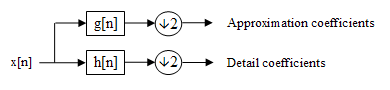
\includegraphics[width=0.5\linewidth]{wave1.png} \\ а)}
\end{minipage}
\begin{minipage}[h!]{1.0\linewidth}
\center{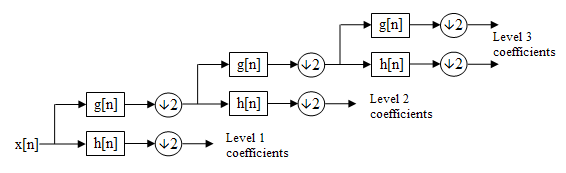
\includegraphics[width=0.5\linewidth]{wave2.png} \\ б)}
\end{minipage}
\caption{Схема действия одно- (а) и трёхуровнего дискретного вейвлет-преобразования.}
\label{wavelet_scheme}
\end{figure}
	\subsubsection{Общий пространственный фильтр}
	\par Общий пространственный фильтр (англ. Common Spatial Pattern Filter, CSP) реализует метод декомпозиции многоканального ЭЭГ сигнала, основанный на обучении по прецедентам.
	\par Рассматривается задача классификации многомерных сигналов на 2 класса. Целью метода является разложение исходного сигнала на аддитивные составляющие таким образом, чтобы максимизировать дисперсию первых компонент и минимизировать дисперсию последених для объектов первого класса и добиться обратной ситуации для объектов второго класса. Матрица декомпозиции может быть найдена в результате одновременной диагонализации выборочных матриц ковариации для каждого из классов. В результате может быть сформирован вектор характерных признаков путём соединения значений некоторого количества первых и последних компонент декомпозированного сигнала.
	\par Метод также может быть обобщён для задачи с количеством классов, больших двух, путём разбиения исходной задачи на бинарные подзадачи с использованием схем <<один против одного>> или <<один против всех>>.



	\subsection{Классификация}
	\par После построения искомого признакового пространства алгоритм, используемый для классификации преобразованных объектов, играет не столь значительную роль. После предобработки и преобразования исходных данных проводится обучение классификатора, после чего обученный классификатор может принимать решение о наличии либо отсутствии волн P300 и, как следствие, о необходимости выполнять действие, предписанное стимулом. Наиболее часто в исследованиях по тематике {\it BCI} используются следующие типы классификаторов.
	\subsubsection{Байесовский классификатор}
	\par Байесовский классификатор — широкий класс алгоритмов классификации, основанный на принципе максимума апостериорной вероятности. Для классифицируемого объекта вычисляются функции правдоподобия каждого из классов, по ним вычисляются апостериорные вероятности классов. Объект относится к тому классу, для которого апостериорная вероятность максимальна.
	\par Байесовский подход к классификации основан на теореме, утверждающей, что если плотности распределения каждого из классов известны, то искомый алгоритм можно выписать в явном аналитическом виде. Более того, этот алгоритм оптимален, то есть обладает минимальной вероятностью ошибок.
	\par На практике плотности распределения классов, как правило, не известны. Их приходится оценивать (восстанавливать) по обучающей выборке. В результате байесовский алгоритм перестаёт быть оптимальным, так как восстановить плотность по выборке можно только с некоторой погрешностью. Зачастую в исследования по тематике создания нейрокомпьютерного интерфейса в качестве функции правдоподобия для объекта используется смесь нормальных распределений.
	\subsubsection{Линейный дискриминант Фишера}
	\par Линейный дискриминант Фишера (ЛДФ) -- особый вариант байесовского классификатора. Рассмотрим задачу классификации на два класса. Предполагается, что обучающая выборка составлена таким образом, что классы распределены по нормальному закону, а матрицы ковариаций классов равны. Простота классификации линейным дискриминантом Фишера -- одно из достоинств алгоритма: в случае с двумя классами в двумерном признаковом пространстве разделяющей поверхностью будет прямая. Если классов больше двух, то разделяющая поверхность будет кусочно-лиинейной.
	\par Данный метод классификации не требует больших вычислительных затрат, а потом является распространённым для онлайн-приложений.
	\subsubsection{Нейронные сети}
	\par Нейронные сети широко используются во многих приложениях, решающих задачу классификации, поскольку обладают высокими гибкостью и эффективностью. Одним из широко применяемых в задачах построения нейрокомпьютерных интерфейсов нейронных сетей является метод обратного распространения ошибки с использованием feed-forward многослойного перцептрона, внутренняя структура которого изображена на рис.~\ref{percep}.
	\subsubsection{Метод опорных векторов}
	\par Метод опорных векторов (англ. SVM, support vector machine) — набор схожих алгоритмов обучения с учителем, принадлежащий к семейству линейных классификаторов. Особым свойством метода опорных векторов является непрерывное уменьшение эмпирической ошибки классификации и увеличение зазора, поэтому метод также известен как метод классификатора с максимальным зазором. Кроме того, на положение разделяющей гиперплоскости в действительности оказывает влияние небольшая часть объектов обучающей выборки. Метод также обобщается на случай нелинейной разделяющей поверхности.
	\par Зачастую используется в исследования по нейрокомпьютерных интерфейсах в силу сводимости к задаче квадратичного программирования и последующей эффективности вычислений.
	\subsubsection{Метод k ближайших соседей}
	\par Метод k ближайших соседей (англ. k-nearest neighbor algorithm, kNN) — метод автоматической классификации объектов. Основным принципом метода ближайших соседей является то, что объект присваивается тому классу, который является наиболее распространённым среди соседей данного элемента. Соседи выбираются из обучающей выборки, и, исходя из ключевого для данного метода значения k, высчитывается, какой класс наиболее многочислен среди них.
	\par Таким образом, если в процессе формирования признакового пространства удалось некоторым образом локализовать объекты каждого из классов в некоторой области пространства, данный метод может быть использован для классификации преобразованных объектов. Кроме того, среди достоинств данного метода ледует упомянуть вычислительную простоту, что делает его простым для использования в онлайн-приложениях.

	\subsection{Критерий качества}
	\par Важным аспектом всякой системы BCI - достигаемая скорость коммуникации. В системах, основанных на распознавании волн P300, данная характеристика зависит от межстимульного интервала, количесва различных стимулов, качества классификации. Чтобы проследить зависимость от перечисленных факторов, будем использовать в качестве метрики для оценивания скорости коммуникации скорость передачи информации (битрейт). Битрейт оценивает количество бит, передаваемых испытуемым системе в единицу времени. Данная характеристика широко используется для оценки работы нейрокомпьютерных интерфейсов, не основанных на волнах P300.
	\par Определим матрицу ошибок для задачи классификации на два класса, разделив эпохи для целевых и нецелевых стимулов на верно и неверно классифицированные:
	\begin{itemize}
	\item
	$a$ -- количество {\bf верно} классифицированных {\bf нецелевых} эпох;
	\item
	$b$ -- количество {\bf неверно} классифицированных {\bf нецелевых} эпох;
	\item
	$c$ -- количество {\bf неверно} классифицированных {\bf целевых} эпох;
	\item
	$d$ -- количество {\bf верно} классифицированных {\bf целевых} эпох.
	\end{itemize}
	Таким образом, можно составить таблицу ~\ref{confusion}. Чувствительностью (англ. true positive rate) называется доля верно классифицированных целевых эпох, специфичностью (англ. false positive rate) -- доля неверно классифицированных нецелевых эпох. Данные величины могут быть вычислены по следующим формулам:
$$TPR = \frac{d}{c+d},$$
$$FPR = \frac{b}{a+b}.$$
	Положим $n_1 = c+d$ - количество целевых эпох, $n_2 = a+b$ - количество нецелевых эпох. Тогда битрейт может быть вычислен по следующей формуле:
$$BR = \frac{d}{n_1 + n_2} * \frac{60}{ITI} * \log_2 (N),$$
где $ITI$ - межстимульный интервал (сек), т.е. промежуток времени между демонстрацией двух последовательных стимулов, $N$ - количество различных визуальных стимулов, используемых в эксперименте.
	\par Кроме указанных величин, точность системы может быть вычислена по формуле:
	$$Accuracy \% = \frac{a+d}{a+b+c+d} * 100 \%.$$
\newpage

\section{Проведение эксперимента}
\subsection{Парадигма эксперимента}
	\par Как правило, в исследованиях на основе визуальных стимулов используется следующая схема получения данных:
	\begin{itemize}
	\item
	Испытуемому в течение $t_1$ секунд демонстрируется визуальный стимул либо ментальное задание, которое предстоит выполнить. 
	\item
	В течение $t_2$ секунд испытуемый сосредотачивает внимание на визуальном стимуле либо выполняет указанное ментальное задание. Кроме того, в процессе этого действия происходит запись данных.
	\item
	Визуальный стимул перестаёт демонстрироваться испытуемому, проводится краткая пауза для восстановления расслабленного состояния и подготовки к следующей итерации.
	\end{itemize}

	\par После изучения материалов по исследуемой тематике и различных видов парадигм, используемых для тестирования применимости разработанных систем управления с использованием нейрокомпьютерных интерфейсов, было принято решение провести две серии эксериментов, использующих различные виды визуальных стимулов. 
	\par Получение данных производилось следующим образом. Испытуемый располагался лицом к монитору компьютера с устройством {\it Emotiv EPOC}, расположенным на голове. На экране монитора было изображено квадратное поле, разбитое на 100 равных квадратов прямыми, параллельными его сторонам, путём деления каждой стороны на 10 равных отрезков. Каждый из квадратов является возможным положением курсора на экране компьютера. Целью испытуемого являлось управление курсором в виде голубого квадрата, расположенного на экране компьютера, от начального до обозначенного конечного положения. Четыре визуальных стимула выделялись на экране последовательно случайным образом, в каждый момент времени было выделено не более одного визуального стимула. В первой серии экспериментов в качестве визуальных стимулов выступали изображения стрелок, отвечающих четырём возможным направлениям движения курсора (вверх, вниз, влево, вправо); во второй серии экспериментов использовались кнопки с текстом, описывающим одно из указанных направлений движения. Испытуемый должен был сконцентрировать внимание на стимуле, отвечающем желаемому направлению движения (целевом стимуле с вероятностью появления 25\%), и игнорировать остальные стимулы, отвечающие нежелательным направлениям движения курсора (нецелевые стимулы с вероятностью появления 75\%).
	\par Назовём {\it пробой} последовательность из выделения некоторого визуального стимула в течение 250 мс, а также последующие 1250 мс, необходимые для обработки, классификации данных, генерации и выполнения перемещения курсора. Интервал между двумя выделениями стимулов был установлен равным 2.5 с, включая время, необходимое на обработку и классификацию данных. Назовём {\it сессией} последовательность проб, предпринятых для достижения курсором целевого положения.
	\par Запись ЭЭГ осуществлялась с частотой дискретизации 128 Гц (с внутренней частотой дискретизации устройства 2048 Гц и последующей первичной обработкой) при помощи устройства {\it Emotiv EPOC}. При записи данных устройство находилось в двух различных положениях: положение по умолчанию и инверсированное положение. В положении по умолчанию были использованы данные 10 сенсоров (F3, FC5, T7, P7, O1, O2, P8, T8, FC6, и F4), поскольку данное подмножество обеспечивает покрытие части скальпа, отвечающей за P300-волны. В инверсированном положении были использованы данные 8 сенсоров (FC6, F4, P8, AF4, AF3, F3, P7 и FC5), поскольку они покрывают центральную часть скальпа, которая считается областью, наиболее активно отвечающей за генерацию P300-волн. Положения указанных сенсоров на голове человека изображены на рис.~\ref{position}.

\begin{figure}[h!]
\begin{minipage}[h!]{0.48\linewidth}
\center{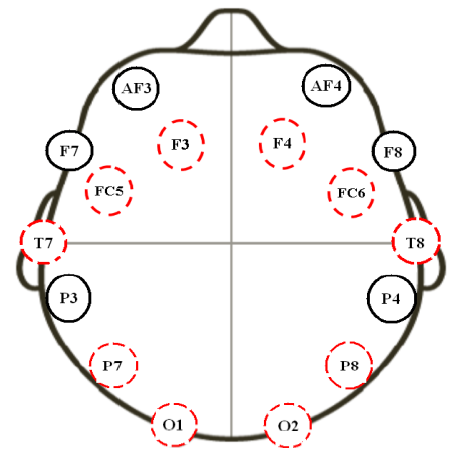
\includegraphics[width=1\linewidth]{default.png} \\ а)}
\end{minipage}
\hfill
\begin{minipage}[h!]{0.5\linewidth}
\center{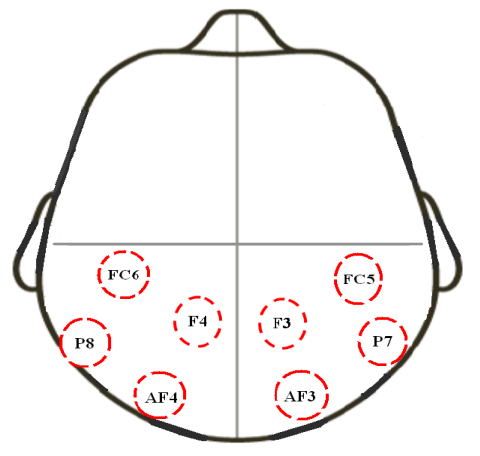
\includegraphics[width=1\linewidth]{inverse.png} \\ б)}
\end{minipage}
\caption{Положения сенсоров для положения устройства по умолчанию (а) и инверсированного положения (б).}
\label{position}
\end{figure}


\subsection{Схема эксперимента}
	\par Самая распространённая схема эксперимента в нейрокомпьютерных интерфейсах, основанных на выявлении волн P300, предполагает, что ответ на целевой стимул не зависит от конкретного стимула, в связи с этим классификация является эффективным методом распознавания целевых и нецелевых стимулов. Тем не менее, некоторые исследования, в частности ..., описывают применение отдельных классификаторов и демонстрируют, что таким образом производительность системы может быть повышена. В связи с этим было решено применить оба подхода и сравнить полученные результаты.
	\par Схема эксперимента для каждого испытуемого состояла из двух частей: предобучение и тестирование в режиме реального времени. В процессе предобучения пользователю необходимо произвести предписанную последовательность действий, описанную ниже, позволяющую собрать некоторое количество данных, используемых для обучения классификатора. В процессе тестирования в режиме реального времени пользователю необходимо производить похожую процедуру, однако полученные данные для каждого из стимулов обрабатываются и классифицируются при помощи предобученного классификатора в тот же момент времени, а также принимается решение о наличии или отсутствии P300-волн и, соответственно, необходимости перемещения курсора в соответствующем направлении.
	\par {\bf Процесс предобучения}
	\par Для функционирования обоих методов необходимо проведение процедуры предобучения отдельно для каждого испытуемого (в силу физиологических различий, ненадёжной фиксации устройства на голове человека, изменения потенциала тела человека с течением времени и т.д.). Предобучение проводится по следующей схеме:
	\begin{itemize} 
	\item
	Испытуемый концентрирует внимание на фиксированном визуальном стимуле в течение 8 раундов.
	\item
	Раунд представляет из себя следующую последовательность действий. В течение раунда каждый из 4 визуальных стимулов, отвечающих возможным направлениям движения курсора, выделяется в течение 250 мс, затем следует период ожидания продолжительностью 2.25 с. 
	\item
	После 8 раундов процесс останавливается на 10 секунд для восстановления расслабленного состояния и подготовки к следующей серии раундов, а затем проводятся раунды для следующего визуального стимула до тех пор, пока не состоялись раунды для всех имеющихся стимулов.
	\item
	Таким образом, обучающая сессия состоит из 32 раундов записи ЭЭГ, содержащих 32 эпохи целевых данных и 96 эпох нецелевых данных. Эпоха представляет собой промежуток времени, содержащий выделение одного из визуальных стимулов и последующий период ожидания вплоть до выделения последующего визуального стимула.
	\item
	Кроме того, также проводится 4 эпохи для записи данных, отвечающих спокойному состоянию испытуемого, т.е. испытуемый расслаблен, а визуальные стимулы не выделяются.
	\item
	Таким образом, количество нецелевых эпох составляет 100. 75\% имеющихся данных используются для обучения классификатора (машины опорных векторов и нейронной сети) для разделения целевых и нецелевых данных. Остальные 25\% данных используются для настройки классификатора в процессе обучения.
	\end{itemize}
	\par Для схемы с использованием отдельных классификаторов используется аналогичный сценарий, однако число раундов для каждого направления равняется 15.

\subsection{Предобработка}
	\par Перед обучением классификатора данные были подвергнуты предобработке. Последовательность действий, применённых к данным, описана ниже. 
	\begin{itemize}
	\item
	{\bf Центрирование данных}
	\par В первую очередь все данные, полученные с каждого электрода, были центрированы с целью нейтрализации постоянного амплитудного смещения. Затем среднее значение сигналов, полученных с электродов сравнения, было использовано для референциального монтажа данных. В положении устройства по умолчанию в качестве электродов сравнения были использованы позиции AF3 и AF4, в инверсированном - O1 и O2.
	\item
	{\bf Выделение отдельных проб}
	\par После этого из полученных данных были выделены отдельные пробы продолжительностью 1500 мс. Начало пробы совпадало с началом выделения визуального стимула на экране компьютера, конец пробы приходился на момент через 1500 мс после начала выделения стимула (250 мс выделения визуального стимула и 1250 мс ожидания). Таким образом, для дальнейшей обработки и определения наличия волн P300 имеются данные, представленные в виде потенциалов, зарегистрированных для 192 моментов времени для каждого из сенсоров, после выделения каждого из визуальных стимулов.
	\item
	{\bf Фильтрация}
	\par Были предприняты попытки использовать несколько типов цифровых фильтров для обработки полученных сигналов: полосно-пропускной фильтр Чебышева 4ого порядка 1ого типа, эллиптический полосно-пропускной фильтр, фильтр с конечной импульсной характеристикой.
	\end{itemize}
	{\bf ICA}
	\par К данным ЭЭГ, подвергнутым фильтрации, был применен метод независимых компонент для извлечения независимых источников. Была использована реализация алгоритма FastICA для {\tt MATLAB}. Описание алгоритма было представлено в предыдущих разделах. Более подробно алгоритм описан в (...).
	\subsection{Отбор признаков}
	\par В (Пиччоне) был использован fuzzy control method для отбора признаков, наиболее точно отбирающие независимые компоненты, похожие на P300-волны, для дальнейшей классификации. Другие исследования используют неавтоматический метод отбора признаков. Поскольку в данной работе используется коммерческое BCI-устройство с высоким уровнем шума в получаемых данных, нет возможности ожидать наличия среди полученных независимых компонент наличие близкой к P300-волне, наподобие полученных в исследовании (Пиччоне). Кроме того, данный метод существенно увеличивает время обработки данных. В исследовании (Ванг и Джемс) показано, что результирующие компоненты ICA, отличные от P300-волн, практически неотличимы для целевых и нецелевых проб, поскольку они являются компонентами одних и тех же источников артефактов в одинаковых условиях. Для первого подхода к компонентам, полученные при помощи метода независимых компонент, применяется дискретное вейвлет-преобразование 3его порядка, где коэффициенты аппроксимации представляют собой  энергию сигнала в полосе P300-волн, включающих энергию сигнала в дельта-, тета- и части альфа-ритмов, как предложено в некоторых исследованиях. Для второго подхода ДВП применяется непосредственно к данным ЭЭГ. Для обоих подходов был использован вейвлет Добеши, поскольку он широко распространён в литературе для подобных целей. Результирующие коэффициенты аппроксимации были использованы в качестве результирующих признаков и были конкатенированы в единые вектора. Результирующая размерность признакового представления объектов равнялась $N_e \times N_f,$ где $N_e$ -- количество компонент или электродов, $N_f$ - количество признаков в одной пробе. Кроме аппроксимирующих коэффициентов, были также использованы 9 морфологических коэффициентов. Таким образом, $N_f = 18 + 9 = 27.$
	{Нормировка}
	\par Отобранные признаки нормировались .....

\subsection{Классификация}
	\par После предобработки и выделения признаков проводится обучение классификатора и валидация, как описано выше. ....

Тестирование в режиме реального времени
	\par ляляля

\newpage

\section{Результаты}
	\par 

\subsection{Обсуждение и~выводы}
Приводятся выводы: 
в~какой степени результаты экспериментов согласуются с~теорией? 
Достигнут ли желаемый результат? 
Обнаружены ли какие-либо факты, не~нашедшие объяснения, и~которые нельзя списать на «грязный» эксперимент?

Обсуждаются основные отличия предложенных методов от известных ранее. 
В~чем их преимущества? 
Каковы границы их применимости? 
Какие проблемы удалось решить, а~какие остались открытыми? 
Какие возникли новые постановки задач?

\section{Заключение}

В~квалификационных работах последний раздел нужен для того, чтобы 
конспективно перечислить основные результаты, полученные лично автором. 

Результатами, в~частности, являются:
\begin{itemize}
\item 
    Предложен новый подход к\dots
\item 
    Разработан новый метод\dots, позволяющий\dots
\item 
    Доказан ряд теорем, подтверждающих (опровергающих), что\dots
\item 
    Проведены вычислительные эксперименты\dots,
    которые подтвердили / опровергли / привели к~новым постановкам задач.
\end{itemize}
    
Цель данного раздела: доказать квалификацию автора. 
Даже беглого взгляда на заключение должно быть достаточно, чтобы стало ясно: 
автору удалось решить актуальную, трудную, ранее не~решённую задачу, 
предложенные автором решения обоснованы и~проверены.

Иногда в~Заключении приводится список направлений дальнейших исследований.

\newpage

\renewcommand{\bibname}{Список литературы}
\addcontentsline{toc}{section}{\bibname}


\def\BibUrl#1.{}\def\BibAnnote#1.{}
%\def\BibUrl#1{\\{\footnotesize\tt\def~{\char126} http://#1}}
\bibliographystyle{plain}

\begin{thebibliography}{1}

\bibitem{voron_report}
Воронцов К. В.
\newblock Аддитивная регуляризация тематических моделей коллекций текстовых документов
\newblock {\em Доклады РАН}, (Т.455, №3. C.268-271), 2014.

\bibitem{voron_potap_tutorial_on_ptm}
Potapenko A.~A. Vorontsov K.~V.
\newblock Tutorial on probabilistic topic modeling: Additive regularization for stochastic matrix factorization.
\newblock {\em AIST, Analysis of Images, Social networks and Texts. -- Springer International Publishing Switzerland, 2014. Communications in Computer and Information Science (CCIS)}, (Vol. 436. pp. 29-46.), 2014.

\bibitem{lda}
Blei,~David~M., Ng,~Andrew~Y., Jordan,~Michael~I.
\newblock Latent Dirichlet allocation.
\newblock {\em Journal of Machine Learning Research.}, (3 (4-5): pp. 993-1022), 2003.

\bibitem{voron_others_kdd}
 Konstantin~Vorontsov, Oleksandr~Frei, Murat~Apishev, Peter~Romov, Marina~Dudarenko.
\newblock Non-bayesian additive regularization for multimodal topic modeling of large collections.
\newblock {\em ???}, 2015.

\bibitem{plsa}
Thomas~Hofmann.
\newblock Probabilistic latent semantic indexing.
\newblock {\em Proceedings of the 22nd annual international ACM SIGIR conference on Research and development in information retrieval.}, (Pp. 50-57), 1999.

\bibitem{online_lda}
D.~Blei M.~Hoffman and F.~Bach.
\newblock Online learning for latent dirichlet allocation.
\newblock {\em Neural Information Processing Systems}, 2010.

\bibitem{ad_lda}
P.~Smyth D.~Newman, A.~Asuncion and M.~Welling.
\newblock Online learning for latent dirichlet allocation.
\newblock {\em Neural Information Processing Systems}, 2009.

\bibitem{plda}
Matt~Stanton Wen-Yen~Chen Yi~Wang, Hongjie~Bai and Edward~Y.~Chang.
\newblock Plda: Parallel latent dirichlet allocation for large-scale applications.
\newblock {\em AAIM}, 2009.

\bibitem{plda_plus}
Zhiyuan~Liu, Yuzhou~Zhang, Edward~Y.~Chang, and Maosong~Sun.
\newblock Plda+: Parallel latent dirichlet allocation with data placement and pipeline processing.
\newblock {\em ACM Transactions on Intelligent Systems and Technology, special issue on Large Scale Machine Learning}, 2011.

\bibitem{y_lda}
Alexander~Smola and Shravan~Narayanamurthy.
\newblock An architecture for parallel topic models.
\newblock {\em Very Large Data Bases}, 2010.

\bibitem{mr_lda}
Ke~Zhai, Jordan~Boyd-Graber, Nima~Asadi, Mohamad~Alkhouja.
\newblock Mr. LDA: A Flexible Large Scale Topic Modeling Package using Variational Inference in MapReduce.
\newblock {\em ACM}, 2012.

\bibitem{gensim}
Radim~Rehurek and Petr~Sojka.
\newblock Software framework for topic modelling with large corpora.
\newblock {\em Proc. LREC Workshop on New Challenges for NLP Frameworks}, 2010.

\bibitem{rubin}
T.~N.~Rubin, A.~Chambers, P.~Smyth, and M.~Steyvers.
\newblock Statistical topic models for multi-label document classification.
\newblock {\em Machine Learning}, (vol. 88, no. 1-2, pp. 157-208), 2012.

\end{thebibliography}




\end{document}
